\documentclass[a4paper, 12pt]{article}
\usepackage{graphicx} % Required for inserting images
\usepackage{fullpage}
\usepackage{amsmath}
\usepackage[dvipsnames]{xcolor}
\usepackage{float}
\usepackage{geometry}
\usepackage{biblatex}
\geometry{margin=1in}
\usepackage{enumitem}
\usepackage{parskip}
\usepackage{pgfplots}
\pgfplotsset{compat=1.18}
\usepackage[normalem]{ulem}
\usepackage[version=4]{mhchem}
\usepackage{tikz}
\usepackage{microtype}
\usepackage{gensymb}
\usepackage{caption}
\usepackage{cancel}
\usepackage{nicefrac}

\newcommand{\lab}[1]{\: \text{#1}}
\newcommand{\degC}{$\degree$C \,}
\newcommand{\degF}{$\degree$F \,}
\newcommand{\R}{\left(0.0821 \: \frac{L \cdot atm}{mol \cdot \text{K}}\right)}
\newcommand{\cunits}{$\frac{J}{g \degree \text{C}}$}
\newcommand{\Hf}{$\Delta H_\text{f}$} % heat of formation
\newcommand{\mathHf}{\Delta H_\text{f}} %heat of formation in math mode

\usepackage{hyperref}
\hypersetup{
colorlinks = true,
linkcolor = teal,
citecolor=teal,         % Set color for citations
filecolor=teal,         % Set color for file links
urlcolor=teal           % Set color for URLs
}


\begin{document}

\begin{center}
\textbf{{\Large AP Chem summer homework}} \\
2025-07-31
\end{center}

\setcounter{section}{1}

\section{Math problems}

\begin{enumerate}[label=\alph*.]
    \item $1.81 \times 10^6$
    \item $1.43 \times 10^6$
    \item $2.482 \times 10^{-7}$
    \item $-1.738 \times 10^{-7}$
    \item $6.2 \times 10^{8}$
    \item $2 \times 10^{-3}$
    \item 5
    \item 0.3
    \item $2 \times 10^{-5}$
    \item $\pm 16/15$
    \item $4 \times 10^{-5}$
    \item 4
    \item $-10.68$
    \item
    \begin{gather*}
    x^2 + 0.1x = 2 \times 10^{-8} \\
    x^2 + 0.1x - 2 \times 10^{-8} = 0 \\
    x = \boxed{2 \times 10^{-7}}
    \end{gather*}
    \item 
    \begin{gather*}
    x + y = 3 \\
    x - y = 9 \\
    2x = 12 \\
    \boxed{x = 6}
    \end{gather*}
\end{enumerate}

\section{Significant figures}


\begin{enumerate}[label=\alph*.]
    \item 5
    \item 3
    \item 4
    \item 3
    \item 5
    \item 1
    \item 1
    \item 6
    \item 5
    \item 6
\end{enumerate}

\section{Chapter 1}

\begin{enumerate}[label=\alph*.]
\item 
\begin{figure}[H]
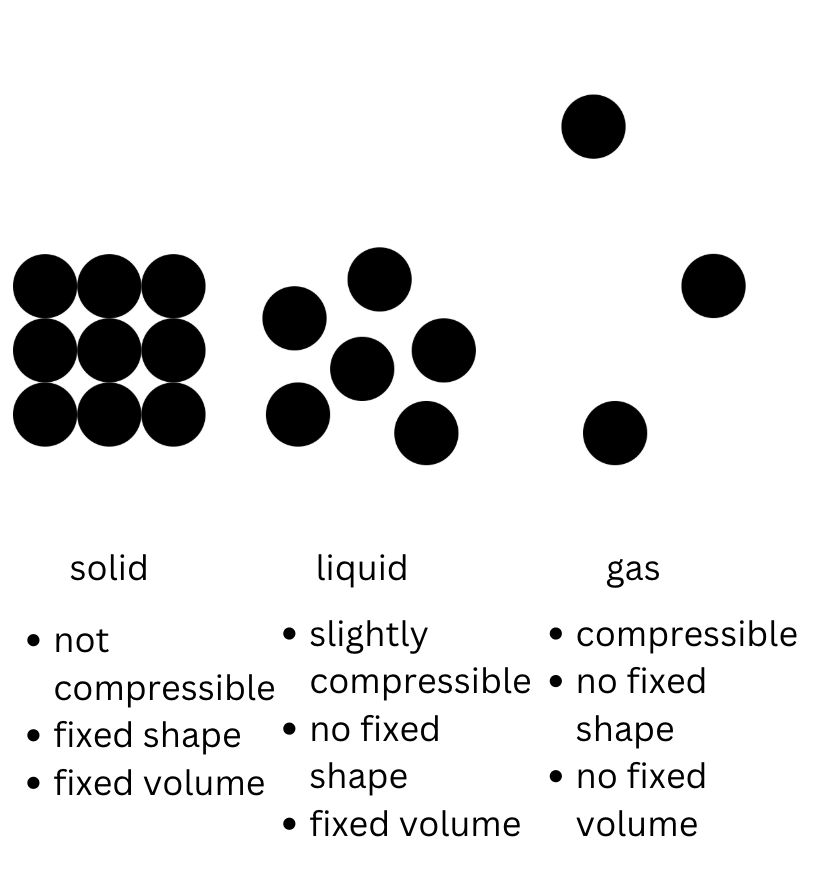
\includegraphics[width=0.5\linewidth]{solidliquidgas}
\end{figure}
\item iii
\item 19\%
\item Dimensional analysis-
\begin{enumerate}[label=\roman*.]
\item
\begin{gather*}
0.069 \lab{nm} = 6.9 \times 10^{-9} \lab{cm} \\
V = \frac{4}{3} \pi (6.9 \times 10^{-9})^3 = 1.38 \times 10^{-24} \lab{cm}^3 \\
\frac{3.35 \times 10^{-23} \lab{g}}{1.38 \times 10^{-24} \lab{cm}^3} = 24.3 \lab{g/cm}^3
\end{gather*}
\item $10^3$; $10^2$; $10^{-3}$; $10^{-6}$; $10^{-9}$
\item $$\frac{330 \lab{minutes}}{1 \lab{day}} \cdot \frac{1 \lab{hour}}{60 \lab{minutes}} = 5.5 \lab{hours/day}$$
\item $$ 1 \lab{year} \times \frac{365 \lab{days}}{1 \lab{year}} \times \frac{24 \lab{hours}}{1 \lab{day}} \times \frac{60 \lab{minutes}}{1 \lab{hour}} \times \frac{60 \lab{seconds}}{1 \lab{minute}} = 3.1536 \times 10^{7} \lab{seconds}$$
\item $$10,000 \lab{L} \times \frac{1000 \lab{ml}}{1 \lab{L}} \times \frac{1 \lab{cm}^3}{1 \lab{ml}} = 10^7 \lab{cm}^3$$
\item $$\frac{1.2 \times 10^9 \lab{gal}}{1 \lab{day}} \times \frac{1 \lab{day}}{24 \lab{hours}} \times \frac{1 \lab{hour}}{60 \lab{minutes}} \times \frac{1 \lab{minute}}{60 \lab{seconds}} = 13888.88 \lab{gallons/second}$$
$$\frac{1 \lab{day}}{1.2 \times 10^9 \lab{gal}} \times \frac{1.3 \times 10^{15} \lab{gal}} = 1.08 \times 10^{6} \lab{days}$$
\item $$2.5 \lab{pounds} \times \frac{453,000 \lab{scales}}{1 \lab{pound}} \times \frac{12 \lab{hours}}{8 \lab{scales}} \times \frac{1 \lab{bee}}{12 \lab{hours}} \approx 10,108 \lab{bees}$$
\end{enumerate}
\item Element: oxygen; compound: water; homogeneous mixture: dish soap; heterogeneous mixture: oil in water; solution: saltwater
\end{enumerate}

\section{Chapter 2}

\begin{enumerate}[label=\alph*.]
\item The mass number is simply the sum of protons plus neutrons in an atom, while average atomic mass is the average of all the masses of all isotopes of an element.  
\item Mass can neither be created nor destroyed
\item
\begin{gather*}
2\ce{H2} + \ce{O2} \to 2\ce{H2O} \\
\text{Available: 4 moles \ce{H2} (2 g/mol) and 1 mole of \ce{O2} (32 g/mol); \ce{O2} is the limiting reactant} \\
\text{Molar mass of \ce{H2O}} = 18 \lab{g/mol} \\
1:2 \: \text{ratio between \ce{O2} and {H2O}} \\
2 \times 18 = 36 \lab{g \ce{H2O}}
\end{gather*}
\item Molar mass of \ce{K2SO4}: 174.26 \lab{g/mol}
\begin{gather*}
\ce{K2}\text{---}2 \cdot 39.1 = 78.2 \lab{g/mol} \\
\ce{S}\text{---}32.06 \lab{g/mol} \\
\ce{O4}\text{---}4 \cdot 16 = 64 \lab{g/mol}
\end{gather*}
Assuming 1 mol, K makes up 78.2 of 174.26 grams
\[\frac{78.2}{174.26} \times 100\% = \boxed{44.88 \%}\]
\item Nucleus: center of the atom consisting of protons and neutrons; orbitals: areas where electrons are most likely to be found, organised by energy level; electrons: particles with negligible mass that are found in the orbitals surrounding the nucleus, adding negative charge; neutrons: a particle found in the nucleus with neutral charge holding protons together
\item Atoms with the same number of protons but different numbers of neutrons (same charge, different mass)
\item C-14
\item Ionic bonding is the bonding of atoms through electrostatic attraction, a result of one atom taking electrons from another to fill both their valence shells; covalent bonding is the bonding of atoms through the sharing of electrons.
\item A chemical formula shows the number of each type of atom in a compound, and a structural formula creates a visual to show where the atoms are connected to each other in space.
\item ion: an atom with a positive or negative net charge due to an unequal number of protons and electrons; cation: an ion with positive charge; anion: an ion with negative charge.
\item Metals are characterised by high conductivity, lustre, and malleability. They lose electrons to nonmetals in ionic bonding. Nonmetals are found on the upper right side of the periodic table, and they take electrons during ionic bonding. They are dull, brittle, and poor conductors of heat and electricity. They also form covalent bonds with each other. Metalloids are elements that fall in between these two sets of characteristics. They are semiconductors and can form both ionic and covalent bonds.
\item Periods are the rows, and groups are the columns on the periodic table.
\item The s-block, p-block, and d-block are the groups that the periodic table is divided into based on the highest energy electron orbital.
\item Group 1, Group 2, Group 7, Group 8
\item \begin{enumerate}[label=\roman*.]
\item Sodium chloride, calcium fluoride, lithium oxide, iron (III) oxide, silver (I) fluoride
\item MgSe, RbI, \ce{Na3P}, \ce{Cu2S}, HgO
\item Ammonium chloride, sodium hydroxide, silver nitrate, manganese (II) carbonate
\item \ce{KBrO3}, \ce{Fe(NO3)3}
\item Phosphorus trichloride, phosphorus pentachloride, sulfur dioxide, carbon dioxide
\item \ce{SO3}, \ce{SF6}, \ce{O2F2}
\item Hydrochloric acid, acetic acid, sulfuric acid
\item \ce{H3PO4}, \ce{HNO3}, \ce{HNO2}
\end{enumerate}
\end{enumerate}

\section{Chapter 3}

\begin{enumerate}[label=\alph*.]
\item 
$19.992 \times 0.9048 + 20.993 \times 0.0027 + 21.991 \times   0.0925 = 20.18 \lab{amu}$
\item There are three different forms of \ce{Br2} with masses of 157.84, 159.84, and 161.84 amu. The middle form is the most abundant because it has the largest peak, and the other two occur in smaller but similar amounts. 
\item An empirical formula shows the simplified ratio of atoms in a compound (for example, \ce{CH2O}) while a molecular formula shows the exact number of atoms in a molecule (\ce{C6H12O6}). 
\item Equations need to be balanced to perform calculations and to make sure that the law of conservation of mass is followed.
\item aqueous (aq), solid (s), liquid (l), gas (g)
\item The ratio of moles in one substance to moles of another in a balanced equation
\item The reactant that limits the amount of product that can be made (and is used up completely)
\item A mixture of ideal proportion where reactants are used completely
\item The theoretical amount of reactant that is expected to be produced
\item The percent yield is the percent of the theoretical yield that was actually produced in the experiment. The formula is 
$$ \text{percent yield} = \frac{\text{actual yield}}{\text{theoretical yield}} \times 100\% $$
\item
\begin{gather*}
\frac{0.2 \lab{g}}{1 \lab{carat}} \times 2.5 \lab{carats} = 0.5 \lab{g} \\
0.5 \lab{g} \times \frac{1 \lab{mol}}{12.011 \lab{g}} = 0.0416 \lab{mol} \\
0.0416 \lab{mol} \times 6.022 \times 10^{23} \lab{atoms/mol} \approx \boxed{2.507 \times 10^{22} \lab{atoms}}
\end{gather*}
\item

\begin{enumerate}[label=\roman*.]
\item 
\begin{gather*}
\text{Molar mass of \ce{Fe2O3}} = 159.687 \lab{g/mol} \\
150 \lab{g} = \frac{1 \lab{mol}}{159.687 \lab{g}} \approx \boxed{0.94 \lab{mol}}
\end{gather*}
\item
\begin{gather*}
\text{Molar mass of \ce{NO2}} = 46.01 \lab{g/mol} \\
10 \lab{mg} \times \frac{1 \lab{g}}{1000 \lab{mg}} \times \frac{1 \lab{mol}}{46.01 \lab{g}} \approx \boxed{0.000217 \lab{mol}}
\end{gather*}
\item
\begin{gather*}
1.5 \times 10^{16} \lab{molecules} \times \frac{1 \lab{mol}}{6.022 \times 10^{23} \lab{molecules}} \approx \boxed{2.5 \times 10^{-1} \lab{mol}}
\end{gather*}
\end{enumerate}
\item
\begin{enumerate}[label=\roman*.]
\item Molar masses: \ce{CH2O} = 30.026 g/mol; C = 12.011 g/mol; 2H = 2.016 g/mol; O = 16 g/mol
\begin{gather*}
\frac{12.011}{30.026} = 40.00\% \lab{C} \\
\frac{2.016}{30.026} = 6.71\% \lab{H} \\
\frac{16}{30.026} = 53.29\% \lab{O}
\end{gather*}
\item same as i. same empirical formula
\item same as i. and ii. also same empirical formula
\end{enumerate}
\item Compound is 48.64\% C (12.011 g/mol), 8.16\% H (1.008 g/mol), 43.2\% O (16 g/mol). Assuming a mass of 100g---
\begin{gather*}
48.64 \lab{g C} \times \frac{1 \lab{mol}}{12.011 \lab{g C}} = 4.05 \lab{mol C} \\
8.16 \lab{g H} \times \frac{1 \lab{mol}}{1.008 \lab{g H}} = 8.10 \lab{mol H} \\
43.2 \lab{g O} \times \frac{1 \lab{mol}}{16 \lab{g O}} = 2.70 \lab{mol O}
\end{gather*}
Mole ratio:
\begin{gather*}
4.05/2.70 = 1.5 \\
8.10/2.70 = 3.0 \\
2.70/2.70 = 1.0
\end{gather*}
As whole numbers:
\begin{gather*}
1.5 \times 2 = 3 \\
3.0 \times 2 = 6 \\
1.0 \times 2 = 2 \\
\boxed{\ce{C3H6O2}}
\end{gather*}
\item 69.6\% sulfur (32.07 g/mol); 30.4\% nitrogen (14.01 g/mol); molar mass 184 g/mol
Empirical:
\begin{gather*}
69.6 \lab{g S} \times \frac{1 \lab{mol}}{32.07 \lab{g}} = 2.17 \lab{mol S} \\
30.4 \lab{g N} \times \frac{1 \lab{mol}}{14.01 \lab{g}} = 2.17 \lab{mol N} \\
\boxed{\ce{SN}}
\end{gather*}
Molecular:
\begin{gather*}
0.696 \times \frac{184 \lab{g}}{1 \lab{mol}} \times \frac{1 \lab{mol}}{32.07 \lab{g}} = 4 \\
0.304 \times \frac{184 \lab{g}}{1 \lab{mol}} \times \frac{1 \lab{mol}}{14.01 \lab{g}} = 4 \\
\boxed{\ce{S4N4}}
\end{gather*}
\item 
\begin{itemize}
\item $\ce{6KO2_{(s)}} + \ce{4H2O_{(l)}} \to \ce{6KOH_{(aq)}} + \ce{4O2_{(g)}} + \ce{H2O2_{(aq)}}$
\item $\ce{Fe2O3_{(s)}} + \ce{6HNO3_{(aq)}} \to \ce{2Fe(NO3)3_{(aq)}} + \ce{3H2O_{(l)}}$
\item $\ce{4NH3_{(g)}} + \ce{5O2_{(g)}} \to \ce{4NO_{(g)}} + \ce{6H2O_{(g)}}$
\item $\ce{PCl5_{(l)} + 4H2O_{(l)} \to H3PO4_{(aq)} + 5HCl_{(g)}}$
\item $\ce{2CaO_{(s)} + 5C_{(s)}} \to \ce{2CaC2_{(s)} + CO2_{(g)}}$
\item $\ce{6MoS2_{(s)} + 21O2_{(g)}} \to \ce{6MoO3_{(s)} + 12SO2_{(g)}}$
\item $\ce{FeCO3_{(s)} + H2CO3_{(aq)} \to Fe(HCO3)2_{(aq)}}$
\end{itemize}
\item Equation: $\ce{N2_{(g)} + 3H2_{(g)}} \to \ce{2NH3_{(g)}}$

Molar mass of \ce{N2} = 28.014 \lab{g/mol}; molar mass of \ce{H2} = 2.016 \lab{g/mol}. 1000 g/28.014 g/mol = 35.70 mol \ce{N2} and 500 g/2.016 g/mol = 248.02 mol \ce{H2} are available. 248.02/3 = 82.67; N2 is the limiting reagent

$$35.70 \lab{mol} \: \ce{N2} \times \frac{2 \lab{mol} \: \ce{NH3}}{1 \lab{mol} \: \ce{N2}} \times \frac{17.034 \lab{g} \: \ce{NH3}}{1 \lab{mol} \: \ce{NH3}} \approx \boxed{1216.5 \lab{g} \: \ce{NH3}}$$

\begin{gather*}
35.70 \lab{mol \ce{N2}} \times \frac{3 \lab{mol \ce{H2}}}{1 \lab{mol \ce{N2}}} = 107.1 \lab{mol \ce{H2} needed for reaction} \\
248.02-107.1 = 140.92 \lab{mol \ce{H2}} \times \frac{2.016 \lab{g}}{1 \lab{mol \ce{H2}}} = 284.09 \lab{g \ce{H2} left over}
\end{gather*}
\item $$\ce{2MnO4^-_{(aq)} + 5C2O4^{2-}_{(aq)} + 16H+_{(aq)}} \to \ce{2Mn^{2+}_{(aq)} + 10CO2_{(g)} + 8H2O_{(l)}}$$

$(0.20\ \lab{mol/L})(0.020\ \lab{L}) = 0.0040 \lab{mol \ce{MnO4^-}}$ and $(0.10 \lab{mol/L})(0.050 \lab{L}) = 0.0050 \lab{mol \ce{C2O4^{2-}}}$ available. $0.0040 \times \frac{5}{2} = 0.010\ \lab{mol \ce{C2O4^{2-}}}$ needed to react with all of the $\ce{MnO4^-}$; lim reageant is $\ce{C2O4^{2-}}$

$$0.0050 \lab{mol \ce{C2O4^{2-}}} \times \frac{10 \lab{mol \ce{CO2}}}{5 \lab{mol \ce{C2O4^{2-}}}} = \boxed{0.010 \lab{mol \ce{CO2}}}$$
\end{enumerate}

\section{Additional knowledge}

\begin{enumerate}[label=\alph*.]
\item $1s^22s^22p^6$
\item [Kr]$5s^24d^{10}5p^2$
\item
\begin{figure}[H]
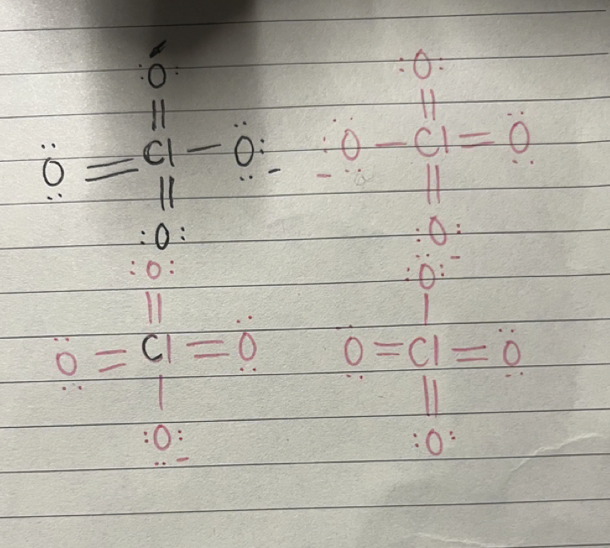
\includegraphics[width=0.5\linewidth]{res}
\end{figure}
\item $sp^2$
\item Trigonal planar; 120 degrees
\end{enumerate}

\section{Questions for review}

Question 6a. had some trouble understanding the table; 6b I don't remember doing in honors chem so I had help from previous AP Chem students on those questions. 7e. I remembered but would like to review VSEPR in more detail; will do before school starts

\end{document}